

\documentclass[handout,18pt]{beamer}
\usepackage{templates/beamerthemekit}
\graphicspath{{./images/}}
\usepackage[citestyle=authoryear,bibstyle=numeric,hyperref,backend=biber]{biblatex}
\addbibresource{templates/example.bib}
\bibhang1em

\author{Benjamin Kenwright}
\title[Introduction to Module]{Introduction to the Module}
\subtitle[Computer Graphics with Vulkan]{Computer Graphics with Vulkan - ZJNU0101600533}
\institute{Zhanjiang Normal University}
\date{}



% \usepackage[backref=page]{hyperref}

\usepackage{hyperref}


%\hypersetup{
%    colorlinks = true, 
%    linkcolor = blue,
%    anchorcolor = blue,
%    citecolor = blue, 
%    filecolor = blue, 
%    %pagecolor = red,
%    urlcolor = blue,
%}

\hypersetup{pdfinfo={
	Author   		= {\author},
	Title    		= {\title},
	Subject  		= {\author},
	Keywords 		= {\title},
	CreationDate 	= {D:2014020220195600},
	Producer		= {\author},
	Creator			= {\author},
}}



\usepackage{graphics}

\begin{document}
\begin{frame} % [plain]
    \titlepage
\end{frame}
    
\begin{frame}{Outline}
    \tableofcontents[pausesections]
\end{frame}
    
\section{Overview of Module}
    
\begin{frame}{Aims and Objectives}
    \pause
    Aims:
    \begin{itemize}
        \item Understand how to build 3D geometric objects
        \item Understand graphics rendering techniques
        \item Understand underpinning mathematics for working in 3D rendering
    \end{itemize}
    \vspace{11pt}
    \pause
    
    Objectives:
    \begin{itemize}
        \item Develop a scene using 3D geometric objects
        \item Utilise graphics rendering techniques within a scene
        \item Utilise mathematical techniques to develop a scene using rendering techniqes
    \end{itemize}
\end{frame}

\begin{frame}{Organisation}
\pause
One lectures per week:
\begin{itemize}
\item \textbf{See Timetable}
\end{itemize}
\pause

One practical per week

The practical sessions are hands-on labs of the concepts discussed in the lectures.

\pause
One tutorial per week

The tutorial will cover mathematical concepts required for the module.

Assessment:
\begin{itemize}
\item Coursework - create scenes in Vulkan
\item Exam - maths, graphics pipeline, rendering concepts
\end{itemize}
\end{frame}

\begin{frame}{Contact}
Questions/Issues

\begin{itemize}
\item Benjamin Kenwright
\item email: bkenwright@ieee.org
\end{itemize}

\vspace{20pt}
\begin{itemize}
\item Open Door Policy 
\item Problems/Help 
\item Within Reason 
\end{itemize}

\end{frame}


\begin{frame}{Ongoing Assessment}
	\pause
	Week 1:
	\begin{itemize}
		\item Recommended Texts/Exercises
        \item Class Quizzes/Discussion
		\item GitHub  
		\item Website/Blog (email me the URL)
	\end{itemize}
	\vspace{11pt}
	\pause
	
	Week 2:
	\begin{itemize}
		\item LaTeX Report (show in Lab)
		\item Tutorial 1 Quiz
	\end{itemize}
	
	Week 3:
	\begin{itemize}
		\item ...
	\end{itemize}
	
\end{frame}


\begin{frame}{Example}
	\pause
	Deliverables...
	\begin{itemize}
		\item peer review
		\item videos 
		\item blog/github
		\item technical reports
		\item presentations
		\item ...
	\end{itemize}
	\vspace{11pt}
	\pause
	
	Your work will be demonstrated to the entire class/university.  Demonstrate high quality competence of computer graphics and software engineering (e.g., ability to write clear well formatted graphics code).
	
\end{frame}


\section{What is Graphics Rendering?}

\begin{frame}{Graphics Rendering}
\pause
Graphics rendering is the use of computational techniques to \\
produce 3D scenes (usually by some form of description file)
\pause        

\vspace{11pt}
Graphics rendering is a major topic in the area of 3D computer graphics.  Other concepts such as animation also fall into the 3D computer graphics area.
\pause

\vspace{11pt}
From our point of view, we are concerned with just creating a 2D image (the computer screen) from the information used to describe a 3D scene.  This module will not concern itself with animation beyond the basic idea of transforming solid objects.
\pause

\vspace{11pt}
Computer graphics were originally developed at Boeing to support GUI development for pilots (in 1961). 
\end{frame}

\begin{frame}{History - Future World}
\begin{columns}
\column{.5\textwidth}
\centering
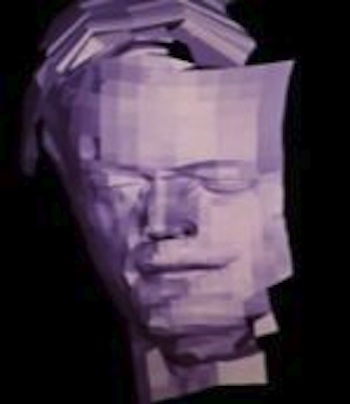
\includegraphics[height=5cm]{futureworld.jpg}
\column{.5\textwidth}

\vspace{20pt}
Future World (1976) was the first film to feature computer generated graphics.  The animated face (left) is simple by today's standards, but was cutting edge in it's day.

\vspace{11pt}
The face was the work of Ed Catmull and Fred Parke.  You will come across the name Catmull quite often in computer graphics (he worked at Lucasfilm, the division which became Pixar, where Catmull is the current president).
\end{columns}
\end{frame}

\begin{frame}{History - Tron}
\begin{columns}
\column{.5\textwidth}
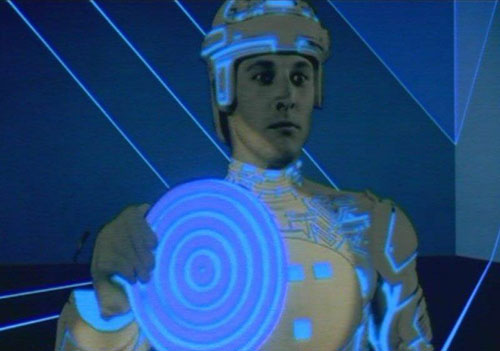
\includegraphics[height=4cm]{tron.jpg}
\column{.5\textwidth}
Tron (1982) was the first film to make extensive use of computer animation techniques.  The computer used to create the generated effects in Tron had only 2MB of memory, and 330MB of storage.

\vspace{11pt}
One innovation from Tron was the development of Perlin noise by Ken Perlin.  This has formed the basis for many procedural content techniques.
\end{columns}
\end{frame}

\begin{frame}{History - Wrath of Khan}
\begin{columns}
\column{.5\textwidth}
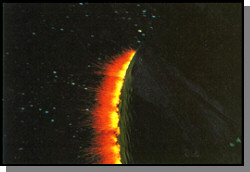
\includegraphics[height=4cm]{khan.jpg}
\column{.5\textwidth}
Star Trek 2: The Wrath of Khan (also 1982) featured the first particle effects in a movie.  Particle effects are used for many fuzzy object effects, such as fire, smoke, and explosions.

\vspace{11pt}
Particle systems are also used for effects such as grass, hair, cloth, and other concepts.  No one really blows anything up anymore, but rather use a particle effect instead.
\end{columns}
\end{frame}

\begin{frame}{History - Toy Story}
\begin{columns}
\column{.5\textwidth}

\includegraphics[height=5.5cm]{toystory.jpeg}
\column{.5\textwidth}

\vspace{10pt}
Toy Story (1995) was the movie that changed everything in computer graphics rendering and animation in movies.  Toy Story is the first fully computer animated movie.

Each frame of the final movie took between 45 minutes and 30 hours to render (well outwith the real-time requirements of games).

One of the key features of the process was Pixar's RenderMan shader language.  Shader languages are fundamental to modern 3D graphics rendering.
\end{columns}
\end{frame}

\begin{frame}{History - Star Wars Episode I}
\begin{columns}
\column{.5\textwidth}

\includegraphics[height=3.5cm]{jarjar.jpg}
\column{.5\textwidth}
Star Wars: Episode I (1999) was the first live action film to use extensive digital effects, especially the use of completely rendered characters, such as Jar Jar Binks.

\vspace{11pt}
Today we don't even notice the effects that appear in films, but it is only recently that we have been able to achieve realistic computer generated effects within live action movies.
\end{columns}
\end{frame}

\begin{frame}{History - Maze War}
\begin{columns}
\column{.4\textwidth}
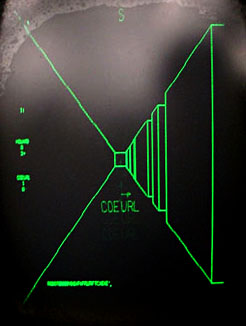
\includegraphics[height=5cm]{mazewar.jpg}
\column{.6\textwidth}

\vspace{10pt}
In parallel with work in movies, video games have also been working towards realistic 3D scenes using computer graphics techniques.

\vspace{11pt}
Unlike movies, games have to operate in real-time (an image has to be generated for a user - a minimum of 24fps is required).

\vspace{11pt}
Maze War (1974) is the first example of a first person style game.  Compare Maze War to something like Call of Duty to see how much has changed.
\end{columns}
\end{frame}

\begin{frame}{History - Battlezone}
\begin{columns}
\column{.5\textwidth}
\centering
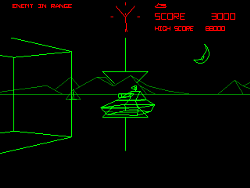
\includegraphics[height=4cm]{battlezone.png}
\column{.5\textwidth}
Battlezone (1980) was the first game considered to have a true 3D world to explore.  Unlike Maze War, the player had freedom of movement in 3D space.

\vspace{11pt}
Battlezone also used a headset in the arcade version.  It is therefore also considered the first virtual reality game as well.
\end{columns}
\end{frame}

\begin{frame}{History - Elite}
\begin{columns}
\column{.5\textwidth}
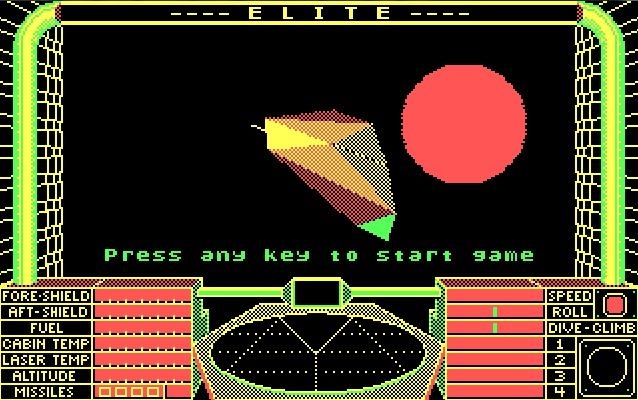
\includegraphics[height=3.5cm]{elite.jpg}
\column{.5\textwidth}

\vspace{15pt}
Elite (1984) brought a 3D universe to explore. Elite is considered one of the cornerstones of using procedural techniques to develop an entire universe to explore, on hardware that had less than 100KB of memory.

Developed by David Braben and Ian Bell while they were at the University of Cambridge.  David Braben currently fronts Frontier Games (Elite 2 was subtitled Frontier), which developed Roller Coaster Tycoon 3.  David is also one of the people behind the Raspberry Pi.
\end{columns}
\end{frame}

\begin{frame}{History - Wolfenstein 3D}
\begin{columns}
\column{.5\textwidth}
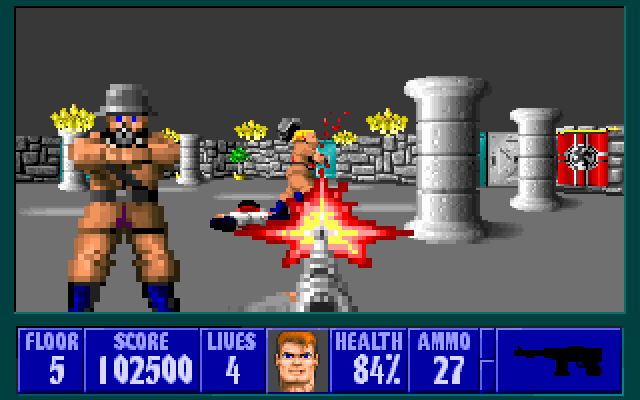
\includegraphics[height=3.5cm]{Wolfenstein3d.png}
\column{.5\textwidth}

\vspace{15pt}
Wolfenstein 3D (1992) essentially created the FPS genre as we know it.

\vspace{11pt}
Wolfenstein 3D did not have fully rendered 3D graphics as we know it today as this was before hardware support for 3D in personal computers.

\vspace{11pt}
Wolfenstein 3D instead used 2D images and traditional approaches for most of the graphics, but utilised a 3D space and some texturing techniques.
\end{columns}
\end{frame}

\begin{frame}{History - Descent}
\begin{columns}
\column{.5\textwidth}
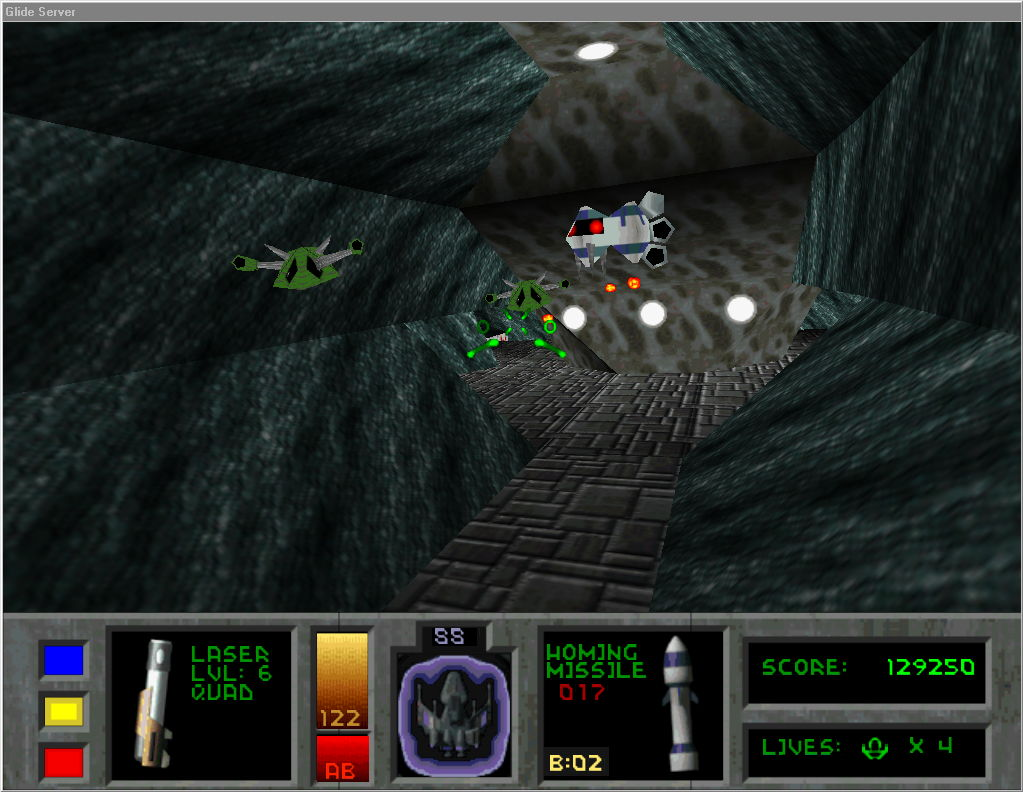
\includegraphics[height=4.5cm]{descent.jpg}
\column{.5\textwidth}
Descent (1995) can be considered the first game to use modern techniques.  The use of polygons and texturing is apparent in Descent.

\vspace{11pt}
The graphical effects in Descent were made possible by the release of the first commercial 3D accelerator aimed at the personal computer market.  The chipset was Voodoo, and it was released by 3Dfx Interactive.
\end{columns}
\end{frame}

\begin{frame}{History - 3Dfx Interactive}
\begin{columns}
\column{.5\textwidth}
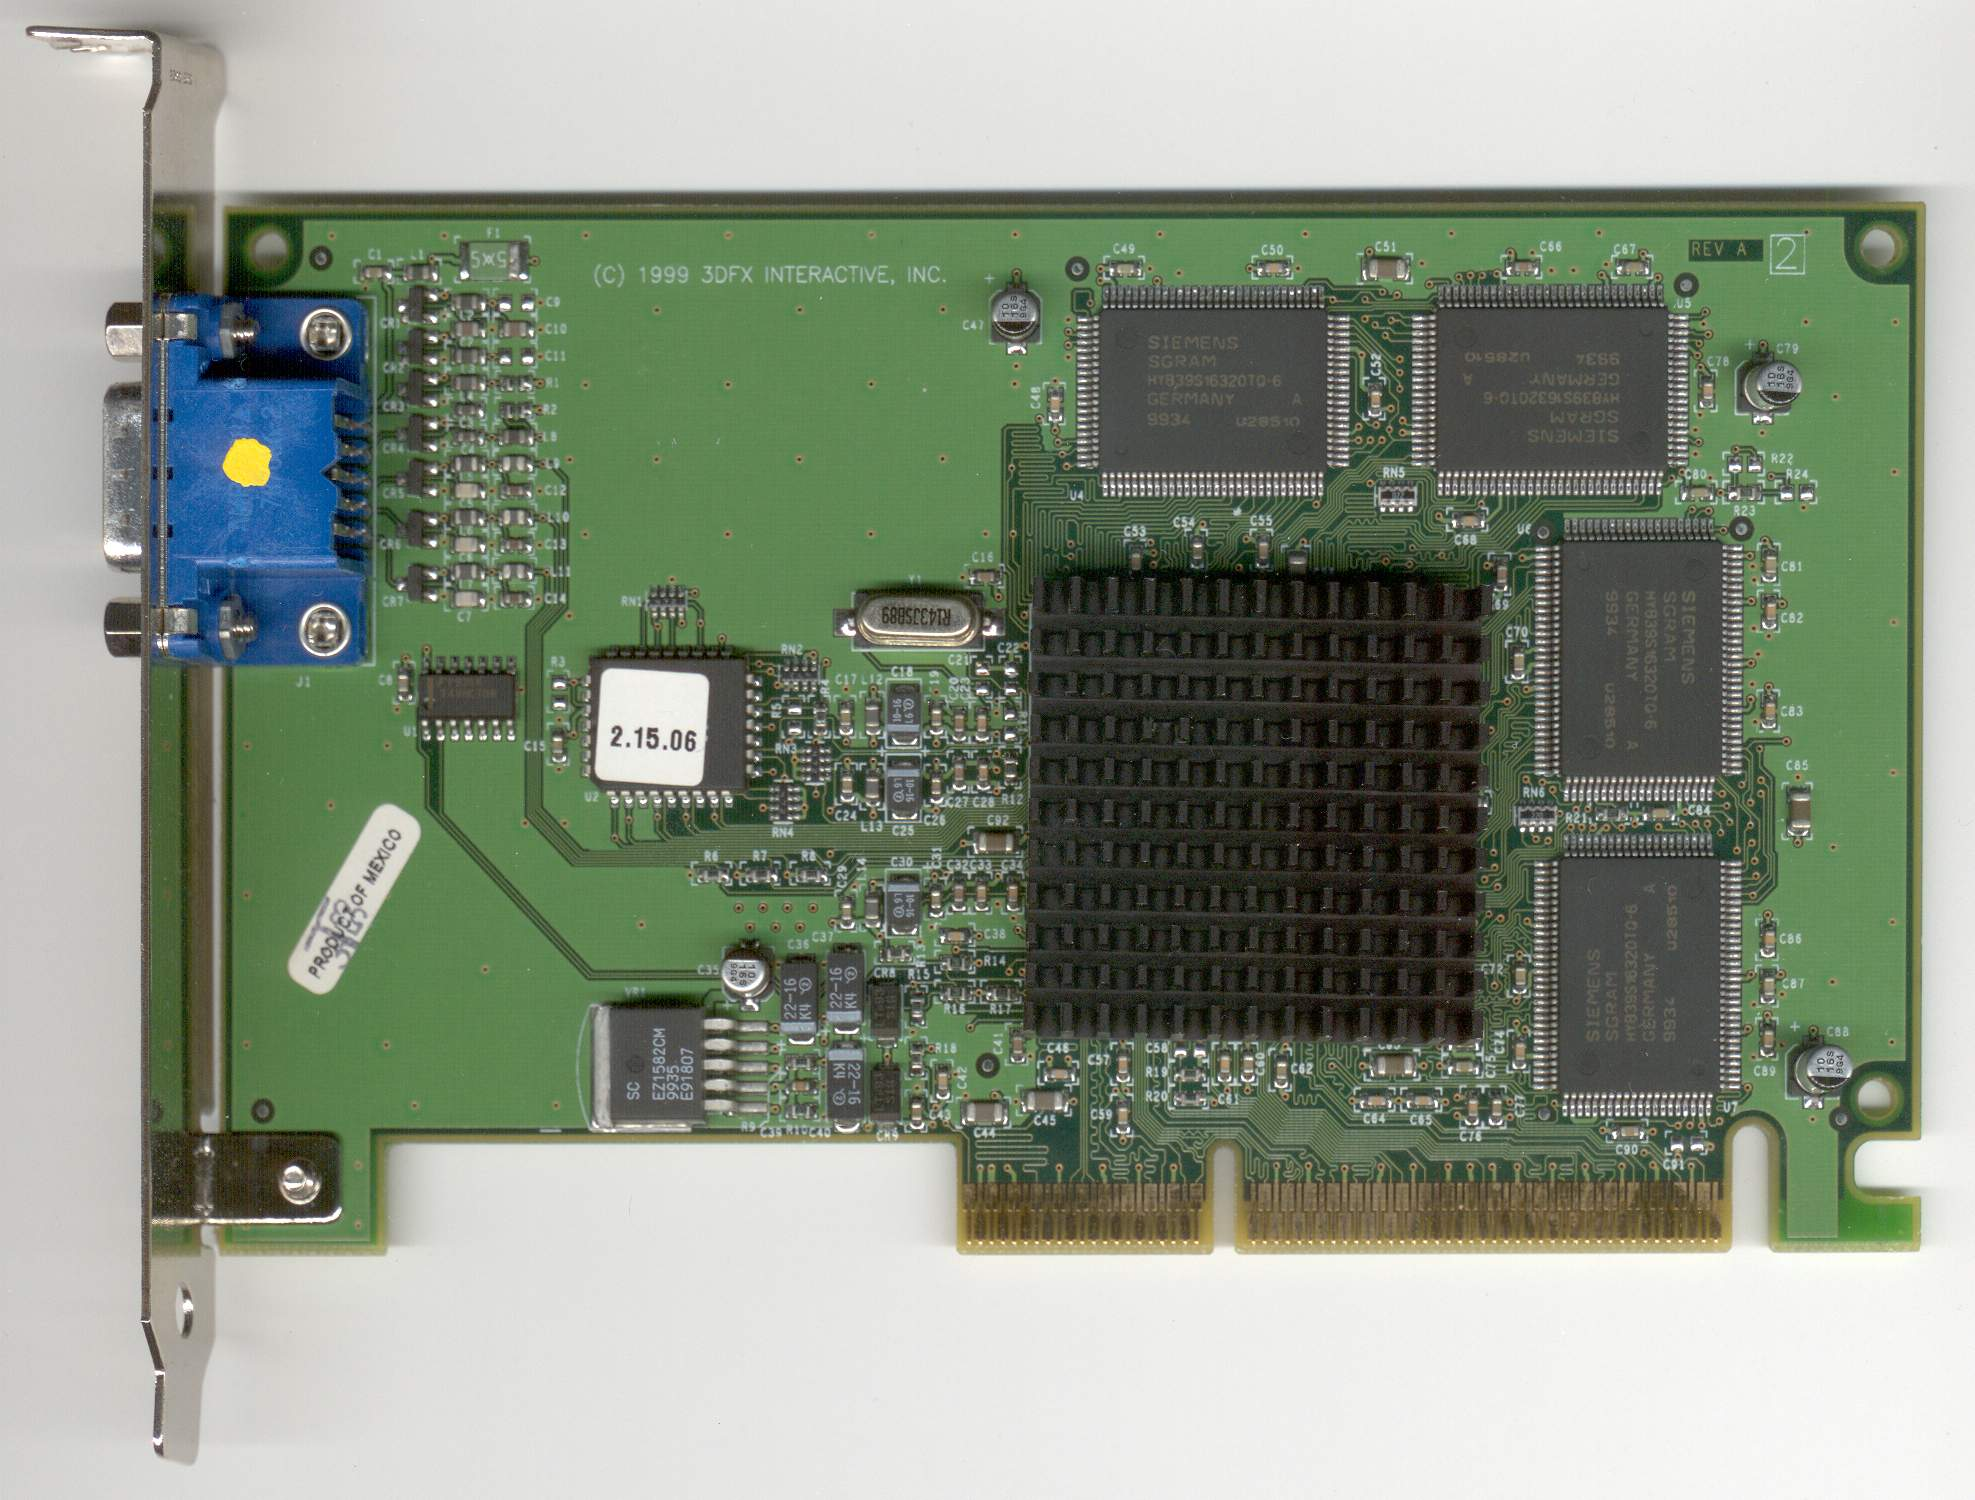
\includegraphics[height=4cm]{voodoo.jpg}
\column{.5\textwidth}
3Dfx Interactive launched the first home use 3D accelerator card in 1996 - due mainly to a reduction in the cost of memory.

\vspace{11pt}
The first cards only had around 4MB of RAM, and had a clock processor of around 50MHz.  Simply having a graphics co-processor though changed everything.

\vspace{11pt}
3Dfx Interactive filed for bankruptcy in 2002.  Most of its intellectual property and staff were taken by Nvidia.
\end{columns}
\end{frame}

\begin{frame}{History - Nvidia and the GPU}
\begin{columns}
\column{.4\textwidth}
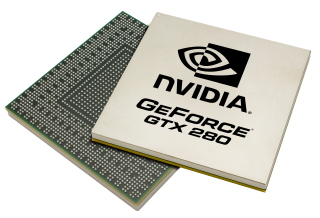
\includegraphics[height=3.5cm]{nvidia.jpg}
\column{.6\textwidth}

\vspace{10pt}
Nvidia coined the phrase Graphics Processing Unit (GPU) in 1999.  The advent of GPUs was the point where modern graphical rendering techniques were born.

\vspace{11pt}
The GPU brought around the concept of texturing and lighting to the consumer market, and therefore games.  By providing hardware accelerated technology for 3D rendering, better visual effects than ever before were possible.

\vspace{11pt}
The basic graphical processing concepts are still in current generation hardware.
\end{columns}
\end{frame}

\begin{frame}{Current Trends}
\pause
Current trends in graphics rendering techniques focus on a mix of better realism (specifically for movies), and better performance (particularly for games).
\pause

\vspace{11pt}
In this module we will be focusing on techniques more suited for real-time rendering techniques.  Although there are techniques which are quite modern, most of our work will actually involve techniques first developed in the 1970s (most game based graphics rendering does this).
\pause

\vspace{11pt}
The main driver behind games based graphics rendering is the limitations of current generation hardware.
\end{frame}

\begin{frame}{Previous Generation Hardware}
\pause
XBox 360 specs:
\begin{itemize}
\item Triple core 3.2 GHz processor
\item 512MB of memory, 10MB of graphics memory
\item Only DirectX 9 compatible
\end{itemize}
\pause

\vspace{11pt}
PS3 specs:
\begin{itemize}
\item Cell Processor (can be thought of as multi-core)
\item 512MB of memory (256MB for graphics).  No dedicated (on board)
graphics memory
\item OpenGL ES 2.0 compatible
\end{itemize}
\pause{}

\vspace{11pt}
Wii specs:
\begin{itemize}
\item 729 MHz processor
\item 88MB of memory, 3MB of graphics memory
\item No programmable shader support
\end{itemize}
\end{frame}

\begin{frame}{Current Generation Hardware}
\pause
XBox One specs:
\begin{itemize}
\item Eight core 1.75 GHz processor
\item 8GB DDR3 memory, 32MB of graphics memory
\item 853 MHz GPU, 768 shader cores
\item DirectX 11.1 compatible
\end{itemize}
\pause

\vspace{5pt}
PS4 specs:
\begin{itemize}
\item Eight core 1.6 GHz processor (supposedly 2.75 GHz capable)
\item 8GB GDDR5 memory.  No dedicated (on board)
graphics memory
\item 800 MHz GPU, 1152 shader cores
\item OpenGL ES 3.0 compatible
\end{itemize}
\pause{}

\vspace{5pt}
Wii specs:
\begin{itemize}
\item Triple core 1.24 GHz processor
\item 2GB DDR3 memory, 32MB of graphics memory
\item 550 MHz GPU, 400 shader cores (rumoured)
\item OpenGL ES 3.0 compatible?
\end{itemize}
\end{frame}

\begin{frame}{Programmable Shaders}
\pause
Currently, most work in modern real-time rendering focuses on utilising the GPU to produce more realistic effects (typically photo-realism).
\pause

\vspace{11pt}
Shader programs are small pieces of code specifically developed to run on the GPU to produce a certain graphical effect.  The GPU is designed to handle graphics rendering using our current approach (e.g. polygon based rendering).
\pause

\vspace{11pt}
More recently, GPUs have enabled general purpose programming through toolkits such as Nvidia's CUDA and OpenCL.  DirectX, OpenGL and Vulkan support compute shaders which enable programmers to utilise the GPU for processes not specifically rendering based.
\end{frame}

\begin{frame}{Photo-realism}
\begin{columns}
\column{.5\textwidth}
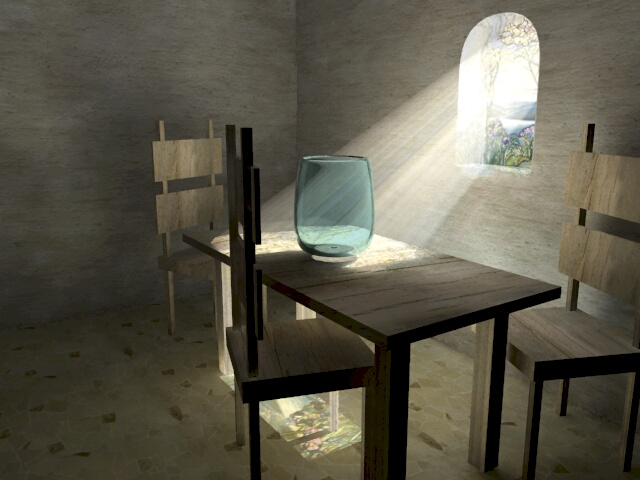
\includegraphics[height=4cm]{photorealism.jpg}
\column{.5\textwidth}

\vspace{15pt}
The goal for graphics rendering is to achieve photo-realism.  This means creating an image that is indistinguishable from a photograph.

\vspace{11pt}
There are already a number of videos reportedly from next-gen engines that support photo-realism - cost of development will likely be a hindrance.

\vspace{11pt}
Realism does lead to the "uncanny valley" effect.
\end{columns}
\end{frame}

\section{Why are we Interested in Graphics Rendering?}

\begin{frame}{Areas}
\pause
There are a number of core areas where graphics rendering is useful:
\begin{itemize}
\pause \item Computer Aided Design (CAD)
\pause \item Computer Generated Images (CGI)
\pause \item Games
\end{itemize}
\pause

\vspace{11pt}
Although most of the ideas we will discuss in the module are applicable to all areas, we will concern ourselves with "real-time" rendering,  which is what we are interested in from a games point of view.
\end{frame}

\begin{frame}{Mathematical Understanding}
\pause
We will also use graphics programming / rendering to better understand 3D space and geometry.
\pause

\vspace{11pt}
We will be covering quite a few ideas in the module, starting from the basics of a geometry system (Euclidean / formal geometry), working through vectors and transformations, 
\pause

\vspace{11pt}
For example, at a minimum, you should feel comfortable with the following:
\[
\vec{p} \cdot \vec{q} = \displaystyle\sum\limits_{i=0}^n p_i q_i
\]
\end{frame}

\section{How does Graphics Rendering Work?}

\begin{frame}{Graphics Cards}
\pause
Graphics programming actually requires us to work on two levels:
\begin{itemize}
\item CPU and application level - where we set up geometry and send commands for how to render it.
\item GPU - where we store geometric data and interpret commands sent from the CPU to render the scene.
\end{itemize}
\pause

\vspace{11pt}
We need to be able to understand the difference between the responsibilities of the CPU and the GPU, particularly with modern approaches to graphics rendering.
\pause

\vspace{11pt}
Initially we will work mainly on the CPU, before moving to the GPU for most rendering operations.
\end{frame}

\begin{frame}{Operations}
\pause
The CPU is responsible for building a 3D scene / model:
\begin{itemize}
\pause \item A scene consists of a number of models
\pause \item A model consists of a number of polygons, textures, etc.
\pause \item A polygon consists of a number of points (vertexes), which contain position, normal data, texture coordinates, etc.
\end{itemize}
\pause

\vspace{11pt}
We used to send this information to the graphics system to render our scene every frame.
\pause

\vspace{11pt}
We now store the information on the graphics card, and tell it how to use the data to render a scene.
\pause

\vspace{11pt}
The number of render images a GPU can produce per second is the "frame rate".  However, the monitor determines how many actual images are shown per second (usually between 60 and 75).
\end{frame}

\begin{frame}{Communication with the GPU}
\pause
In order to communicate with the GPU, we need to use an API:
\begin{itemize}
\item OpenGL (or Vulkan)
\item DirectX (or specifically Direct3D)
\end{itemize}
\pause

\vspace{11pt}
Each API essentially does the same job.  However OpenGL and Vulkan is aimed at general purpose graphics rendering.  DirectX is a aimed at games development, with Direct3D being the rendering part.  Direct3D is still more aimed at the games market than OpenGL/Vulkan.
\pause

\vspace{11pt}
OpenGL/Vulkan is supported on almost all hardware (except the Xbox) - including iOS and Android.  DirectX is only supported on Windows PCs and the Xbox.
\end{frame}

\begin{frame}{Modernisation}
\pause
Reasons to keep the API:
\begin{itemize}
\pause \item Programmers want a stable platform.
\pause \item Programmers want to write one program that will work on all hardware.
\pause \item Game companies want the widest market.
\pause \item GPU manufacturers want backwards compatibility.
\end{itemize}
\pause

\vspace{11pt}
Reasons to update the API:
\begin{itemize}
\pause \item New features can be implemented.
\pause \item GPU vendors can take advantage of hardware features, and exploit the market.
\pause \item Historical features can be a hindrance.
\end{itemize}
\end{frame}

\section{Vulkan}

\begin{frame}{What is Vulkan?}
\pause
Vulkan is a low-level API specifically developed for working with 3D graphics - although recently work has focused on other aspects, such as, compute operations (GPU for calculations other than graphics, like simulations and solving mathematical problems)
\pause

\vspace{11pt}
Vulkan has a number of properties that make it ``useful'':
\begin{itemize}
\item Low level
\item Minimal
\item Does not attempt to be convenient
\item Fast and efficient
\end{itemize}
\pause

\vspace{11pt}
Currently we are at Vulkan 1.0, which is attempting to gain closer interaction with the underlying hardware.
\end{frame}

\begin{frame}{Primitives and Low Level Components}
\pause
Vulkan works with the following low level geometric primitives:
\begin{itemize}
\item Points
\item Lines
\item Triangles
\item Quads
\item Polygons
\end{itemize}
\pause

\vspace{11pt}
Vulkan also supports concepts such as:
\begin{itemize}
\item Colours
\item Normals
\item Texture Coordinates
\end{itemize}
\pause

\vspace{11pt}
Vulkan utilises these values to produce a 3D scene.
\end{frame}

\begin{frame}{Shaders}
\pause
Vulkan supports programmable shaders to enable specific graphical 
effects.
\pause

\vspace{11pt}
Vulkan utilises a bytecode format is called SPIR-V.
GLSL (GL Shader Language) shader language is able to be compiled to this format.
There are also libraries available to support other shader languages.  
The most commonly used other shader language is Nvidia's Cg.
\pause

\vspace{11pt}
We will be working with GLSL extensively as we continue through the 
module.  We will also be looking at different shader types.
\end{frame}

\begin{frame}{Native Applications}
\pause
We will be writing native Vulkan applications (from the ground-up) - including base-classes for Vectors and Matrices to demonstrate an understanding of raw mathematical concepts.
\pause

\vspace{11pt}
While writing libraries from scratch is tedious and time consuming - it enables you to see the underlying concepts close up (instead of ignoring them).
We'll discuss and employ a number of libraries later on when we start to expand our knowledge and implement more advanced features (e.g., model loading libraries, physics libraries, compressions libraries).

\pause

\vspace{11pt}
We aim to develop solutions that are cross platform, as is Vulkan, meaning our applications will work on any desktop/mobile platform (Linux, Windows and Android).
\pause

\vspace{11pt}
We'll also discuss input management, such as, keyboard and mouse support - which is essential for user interaction.
\end{frame}


\begin{frame}{Recommended Reading}
\begin{columns}
\column{.5\textwidth}
\centering
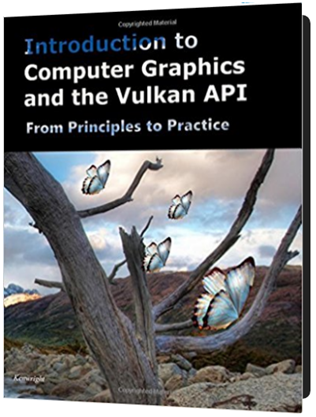
\includegraphics[height=4cm]{book}
\column{.5\textwidth}
Introduction to Computer Graphics and the Vulkan API by Kenwright

\vspace{11pt}
Covers all the major aspects of the module (e.g., introduction to graphical principles and the Vulkan API through to graphical effects like lighting and displacement mapping)

\vspace{11pt}
Read Chapters 1 \& 2 This Week
\end{columns}
\end{frame}




\section{Summary}

\begin{frame}{Summary}
What you should have learnt from this lecture:
\begin{itemize}
\pause \item Graphics rendering has a long history, starting in 
the 1960s at Boeing, through to modern real-time techniques in
modern games.
\pause \item Graphics rendering can support a number of areas - we 
will be focusing on real-time aspects and games.
\pause \item Current generation hardware dictates the current 
quality of computer graphics in games.
\pause \item Shaders and GPGPU are important ongoing directions
\pause \item There are fundamental theoretical reasons we perform
computer graphics in the way that we do.
\pause \item Core concepts of Vulkan, OpenGL and DirectX have lots of common properties/overlap
- Vulkan is the focus of this module (low-level API)
\end{itemize}
\pause

\end{frame}




\begin{frame}{Questions/Discussion}

\end{frame}


\end{document}
